\documentclass[final]{beamer}\usepackage[]{graphicx}\usepackage[]{color}
%% maxwidth is the original width if it is less than linewidth
%% otherwise use linewidth (to make sure the graphics do not exceed the margin)
\makeatletter
\def\maxwidth{ %
  \ifdim\Gin@nat@width>\linewidth
    \linewidth
  \else
    \Gin@nat@width
  \fi
}
\makeatother

\definecolor{fgcolor}{rgb}{0.345, 0.345, 0.345}
\newcommand{\hlnum}[1]{\textcolor[rgb]{0.686,0.059,0.569}{#1}}%
\newcommand{\hlstr}[1]{\textcolor[rgb]{0.192,0.494,0.8}{#1}}%
\newcommand{\hlcom}[1]{\textcolor[rgb]{0.678,0.584,0.686}{\textit{#1}}}%
\newcommand{\hlopt}[1]{\textcolor[rgb]{0,0,0}{#1}}%
\newcommand{\hlstd}[1]{\textcolor[rgb]{0.345,0.345,0.345}{#1}}%
\newcommand{\hlkwa}[1]{\textcolor[rgb]{0.161,0.373,0.58}{\textbf{#1}}}%
\newcommand{\hlkwb}[1]{\textcolor[rgb]{0.69,0.353,0.396}{#1}}%
\newcommand{\hlkwc}[1]{\textcolor[rgb]{0.333,0.667,0.333}{#1}}%
\newcommand{\hlkwd}[1]{\textcolor[rgb]{0.737,0.353,0.396}{\textbf{#1}}}%
\let\hlipl\hlkwb

\usepackage{framed}
\makeatletter
\newenvironment{kframe}{%
 \def\at@end@of@kframe{}%
 \ifinner\ifhmode%
  \def\at@end@of@kframe{\end{minipage}}%
  \begin{minipage}{\columnwidth}%
 \fi\fi%
 \def\FrameCommand##1{\hskip\@totalleftmargin \hskip-\fboxsep
 \colorbox{shadecolor}{##1}\hskip-\fboxsep
     % There is no \\@totalrightmargin, so:
     \hskip-\linewidth \hskip-\@totalleftmargin \hskip\columnwidth}%
 \MakeFramed {\advance\hsize-\width
   \@totalleftmargin\z@ \linewidth\hsize
   \@setminipage}}%
 {\par\unskip\endMakeFramed%
 \at@end@of@kframe}
\makeatother

\definecolor{shadecolor}{rgb}{.97, .97, .97}
\definecolor{messagecolor}{rgb}{0, 0, 0}
\definecolor{warningcolor}{rgb}{1, 0, 1}
\definecolor{errorcolor}{rgb}{1, 0, 0}
\newenvironment{knitrout}{}{} % an empty environment to be redefined in TeX

\usepackage{alltt}
\usepackage[scale=1.20]{beamerposter} % Use the beamerposter package for laying out the poster
\usetheme{confposter} % Use the confposter theme supplied with this template
\setbeamercolor{block title}{fg=DarkOrchid,bg=white} % Colors of the block titles
\setbeamercolor{block body}{fg=black,bg=white} % Colors of the body of blocks
\setbeamercolor{block alerted title}{fg=white,bg=BrewerBlue1} % Colors of the highlighted block titles
\setbeamercolor{block alerted body}{fg=black,bg=dblue!10} % Colors of the body of highlighted blocks
% Many more colors are available for use in beamerthemeconfposter.sty

%-----------------------------------------------------------
% Define the column widths and overall poster size
% To set effective sepwid, onecolwid and twocolwid values, first choose how many columns you want and how much separation you want between columns
% In this template, the separation width chosen is 0.024 of the paper width and a 4-column layout
% onecolwid should therefore be (1-(# of columns+1)*sepwid)/# of columns e.g. (1-(4+1)*0.024)/4 = 0.22
% Set twocolwid to be (2*onecolwid)+sepwid = 0.464
% Set threecolwid to be (3*onecolwid)+2*sepwid = 0.708

\newlength{\sepwid}
\newlength{\onecolwid}
\newlength{\twocolwid}
\newlength{\threecolwid}
\setlength{\paperwidth}{45in} % A0 width: 46.8in
\setlength{\paperheight}{36in} % A0 height: 33.1in
\setlength{\sepwid}{0.01\paperwidth} % Separation width (white space) between columns
\setlength{\onecolwid}{0.24\paperwidth} % Width of one column
\setlength{\twocolwid}{0.464\paperwidth} % Width of two columns
\setlength{\threecolwid}{0.708\paperwidth} % Width of three columns
\setlength{\topmargin}{-0.5in} % Reduce the top margin size
%-----------------------------------------------------------

\usepackage{graphicx}  % Required for including images
\usepackage{booktabs} % Top and bottom rules for tables


\title{Reviewing wildlife biodiversity research from African rangelands} 

\author{Devan Allen McGranahan \inst{1} \and Kevin P. Kirkman \inst{2}}
\institute{\inst{1} School for Natural Resource Sciences\textemdash Range Science Program, North Dakota State University, Fargo, North Dakota USA \and
                      \inst{2} Grassland Sciences Department, University of KwaZulu-Natal, Scottsville, South Africa}
\IfFileExists{upquote.sty}{\usepackage{upquote}}{}
\begin{document}
%\SweaveOpts{concordance=TRUE}


\addtobeamertemplate{block end}{}{\vspace*{2ex}} % White space under blocks
\addtobeamertemplate{block alerted end}{}{\vspace*{2ex}} % White space under highlighted (alert) blocks

\setlength{\belowcaptionskip}{2ex} % White space under figures
\setlength\belowdisplayshortskip{2ex} % White space under equations

\begin{frame}[t] % The whole poster is enclosed in one beamer frame

\begin{columns}[t] % The whole poster consists of three major columns, the second of which is split into two columns twice - the [t] option aligns each column's content to the top

\begin{column}{\sepwid}\end{column} % Empty spacer column

\begin{column}{\onecolwid} % The first column


%	OBJECTIVES

\begin{alertblock}{Overview}
\begin{itemize}
\item African rangelands are diverse. Understanding responses of biodiversity to disturbance is critical to conservation management. \textbf{As ecological theory \& research analytical methods have developed worldwide, has African biodiversity science kept up?}

\item We systematically reviewed primary literature on bird, small mammal, herptofauna, and invertebrate responses to disturbance in African rangelands, \textbf{principally fire and grazing}.

\item Overall, solid understanding of biodiversity response is limited geographically, \& within taxa limited by insufficient replication, lack of experimentation, \& weak community analysis. 

\item \textbf{Spatial \& temporal heterogeneity are overlooked} and should be combined with multivariate analysis of long-term datasets to relate management and disturbance interactions to community assembly and succession. 

\end{itemize}
\end{alertblock}

%	INTRODUCTION

\begin{block}{Review methods}
\small{
\begin{itemize}
\item Web of Science search with disturbance-related wildcard terms graz* OR herbivor*; fire OR burn*; AND africa*
\item Inclusion criteria: Original data on faunal response to treatment/management from rangeland ecosystem
\item Each paper searched backwards/forwards: Bibliographies + "cited by" in Google Scholar (same inclusion criteria)
\end{itemize}}
\begin{table}
\small
\caption{We ranked the analyses we encountered by strength, based on their (1) sensitivity to individual species identity and (2) ability to test dissimilarity among groups or along gradients:}
\begin{tabular}{l l}
\toprule
\textbf{Category} & \textbf{Explanation/description} \\ \midrule
None & univariate responses (ANOVA, t-test) are species-specific \\ \midrule
Very & MANOVA, richness, \& diversity indices (Shannon, \\
weak & Simpson, etc) lack information on species identity  \\ \midrule
Weak & Dissimilarity indices, classification, indicator species\\ 
\midrule
Moderate  & Ordination without testing group dissimilarity \\ \midrule
Strong    & Ordination \& clustering that tests dissimilarity\\ \midrule
Very      & Ordination that tests dissimiliarity among \\
  strong  & groups or along environmental gradient \\ \bottomrule
\end{tabular}
\end{table}

\end{block}

%------------------------------------------------


\end{column} % End of the first column
\begin{column}{\sepwid}\end{column} % Left spacer column

\begin{column}{\twocolwid} % Begin a column two columns wide (column 2)

\begin{columns}[T] % align columns

\begin{column}{0.5\textwidth}
\vspace{-2cm}
\begin{block}{The diversity of biodiversity research in sub-Saharan Africa} \end{block}
\vspace{-1cm}

\begin{knitrout}
\definecolor{shadecolor}{rgb}{0.969, 0.969, 0.969}\color{fgcolor}\begin{figure}

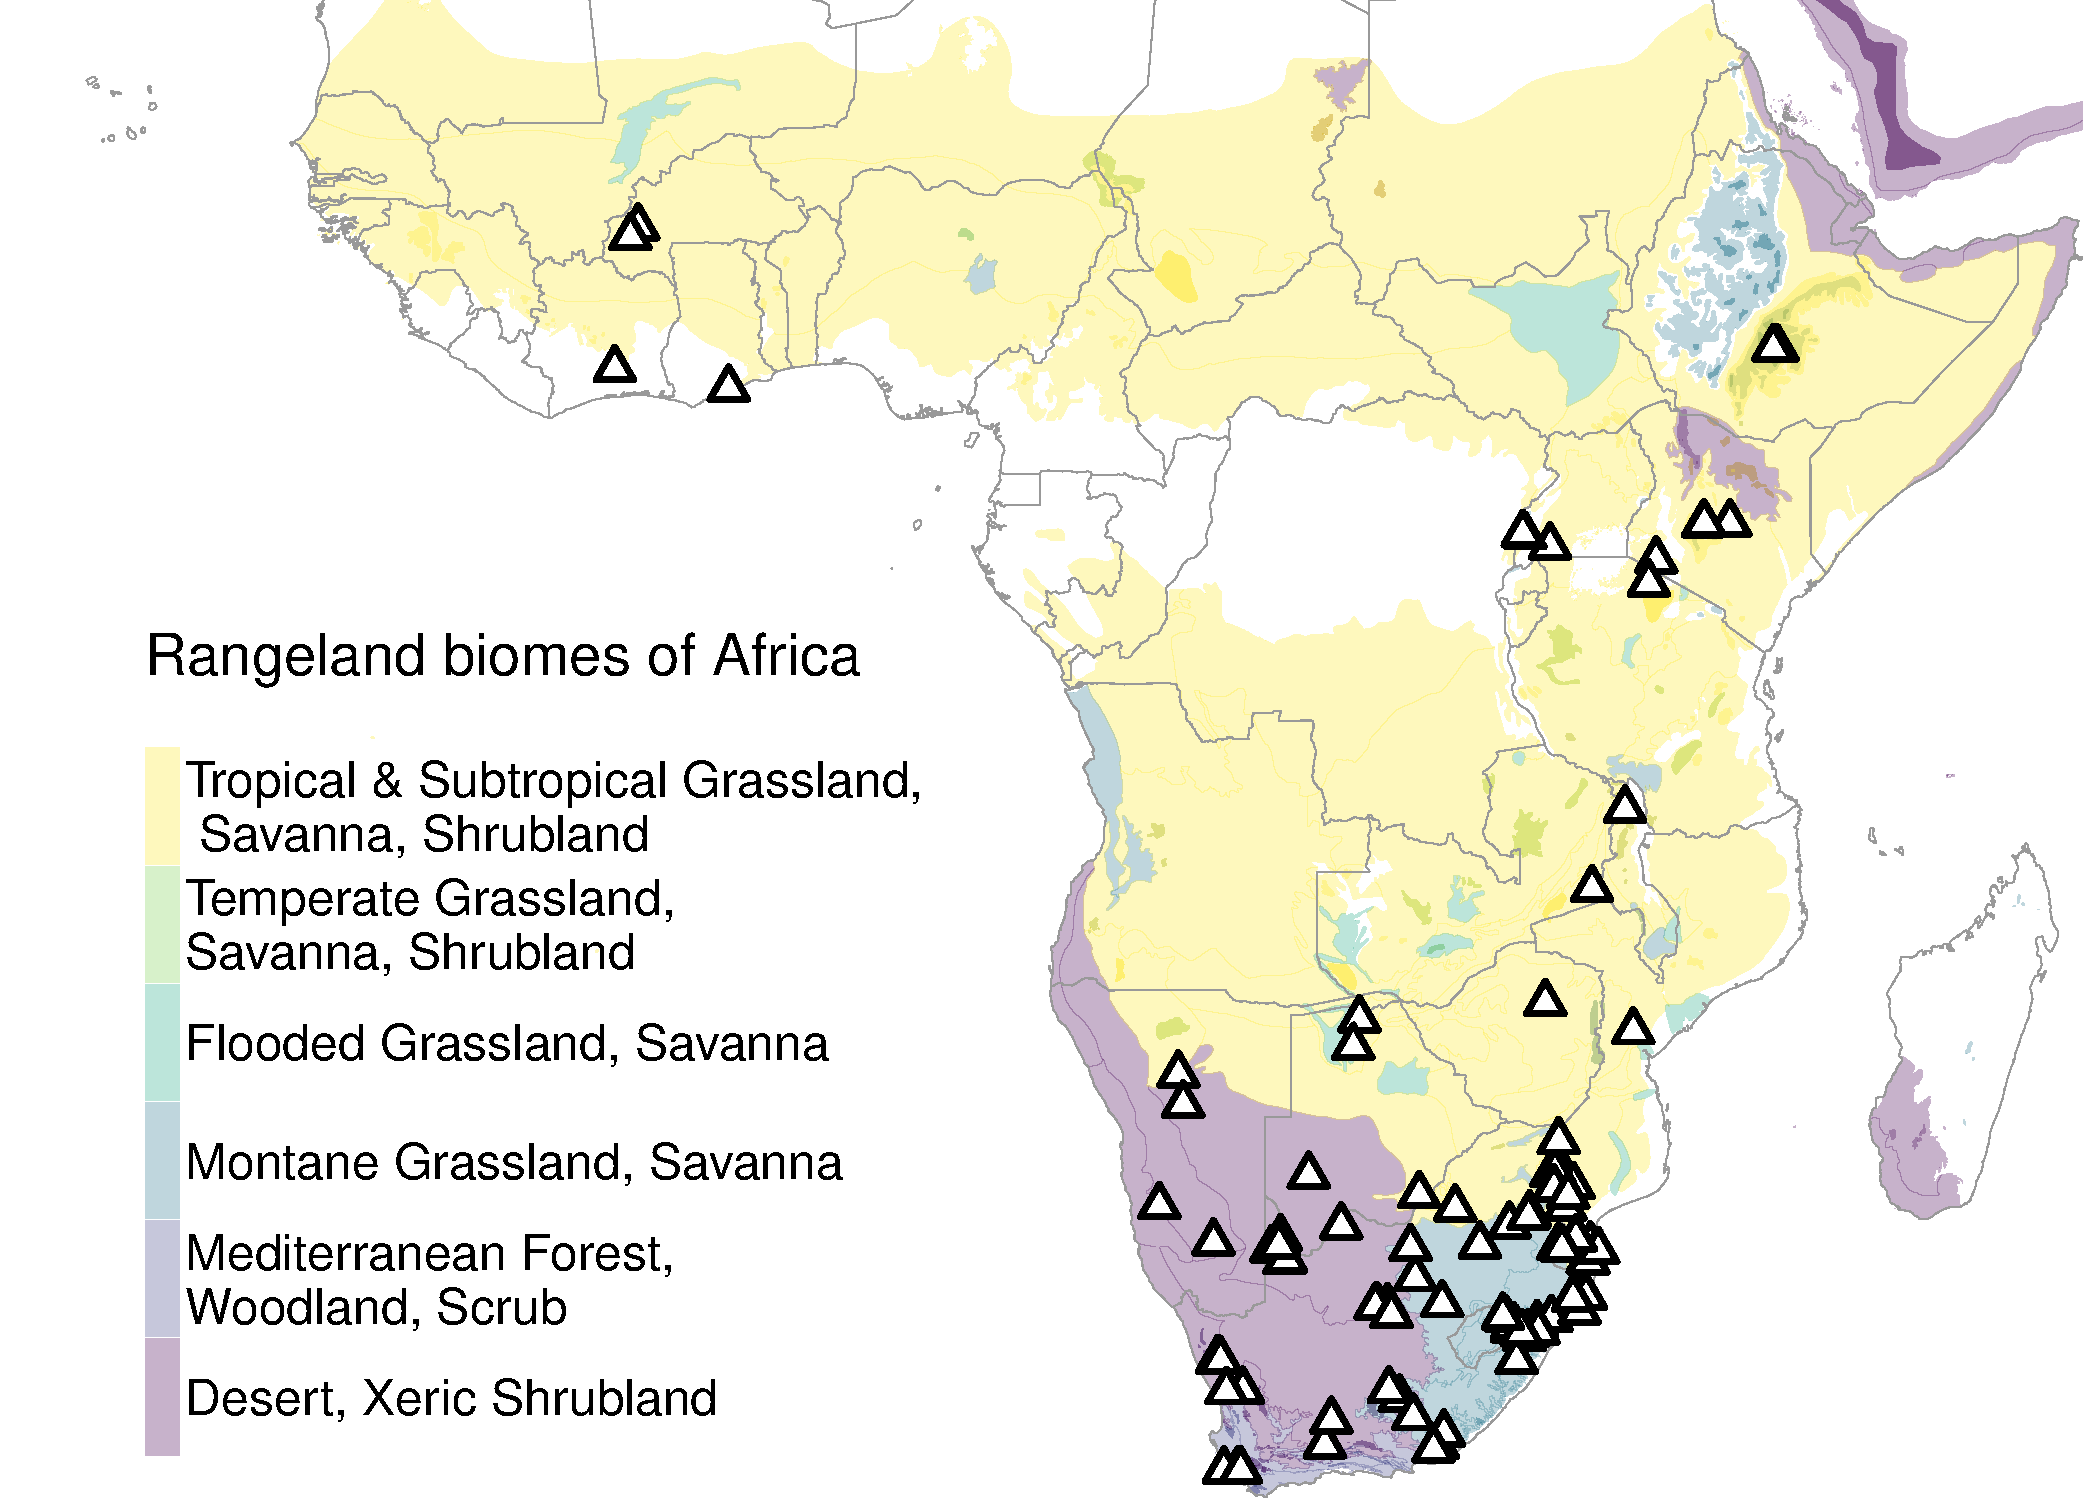
\includegraphics[width=\maxwidth]{figure/beamer-map-1} \hfill{}

\caption[ Location of studies included in review]{ Location of studies included in review}\label{fig:map}
\end{figure}


\end{knitrout}


\end{column}%
\hfill%
\begin{column}{0.45\textwidth}
\vspace{-2cm}
\begin{itemize}
\item Most research comes from South Africa
\item 78\% of studies were observational
\item 64\% were pseudo-replicated or not replicated
\end{itemize}

\begin{knitrout}
\definecolor{shadecolor}{rgb}{0.969, 0.969, 0.969}\color{fgcolor}\begin{figure}

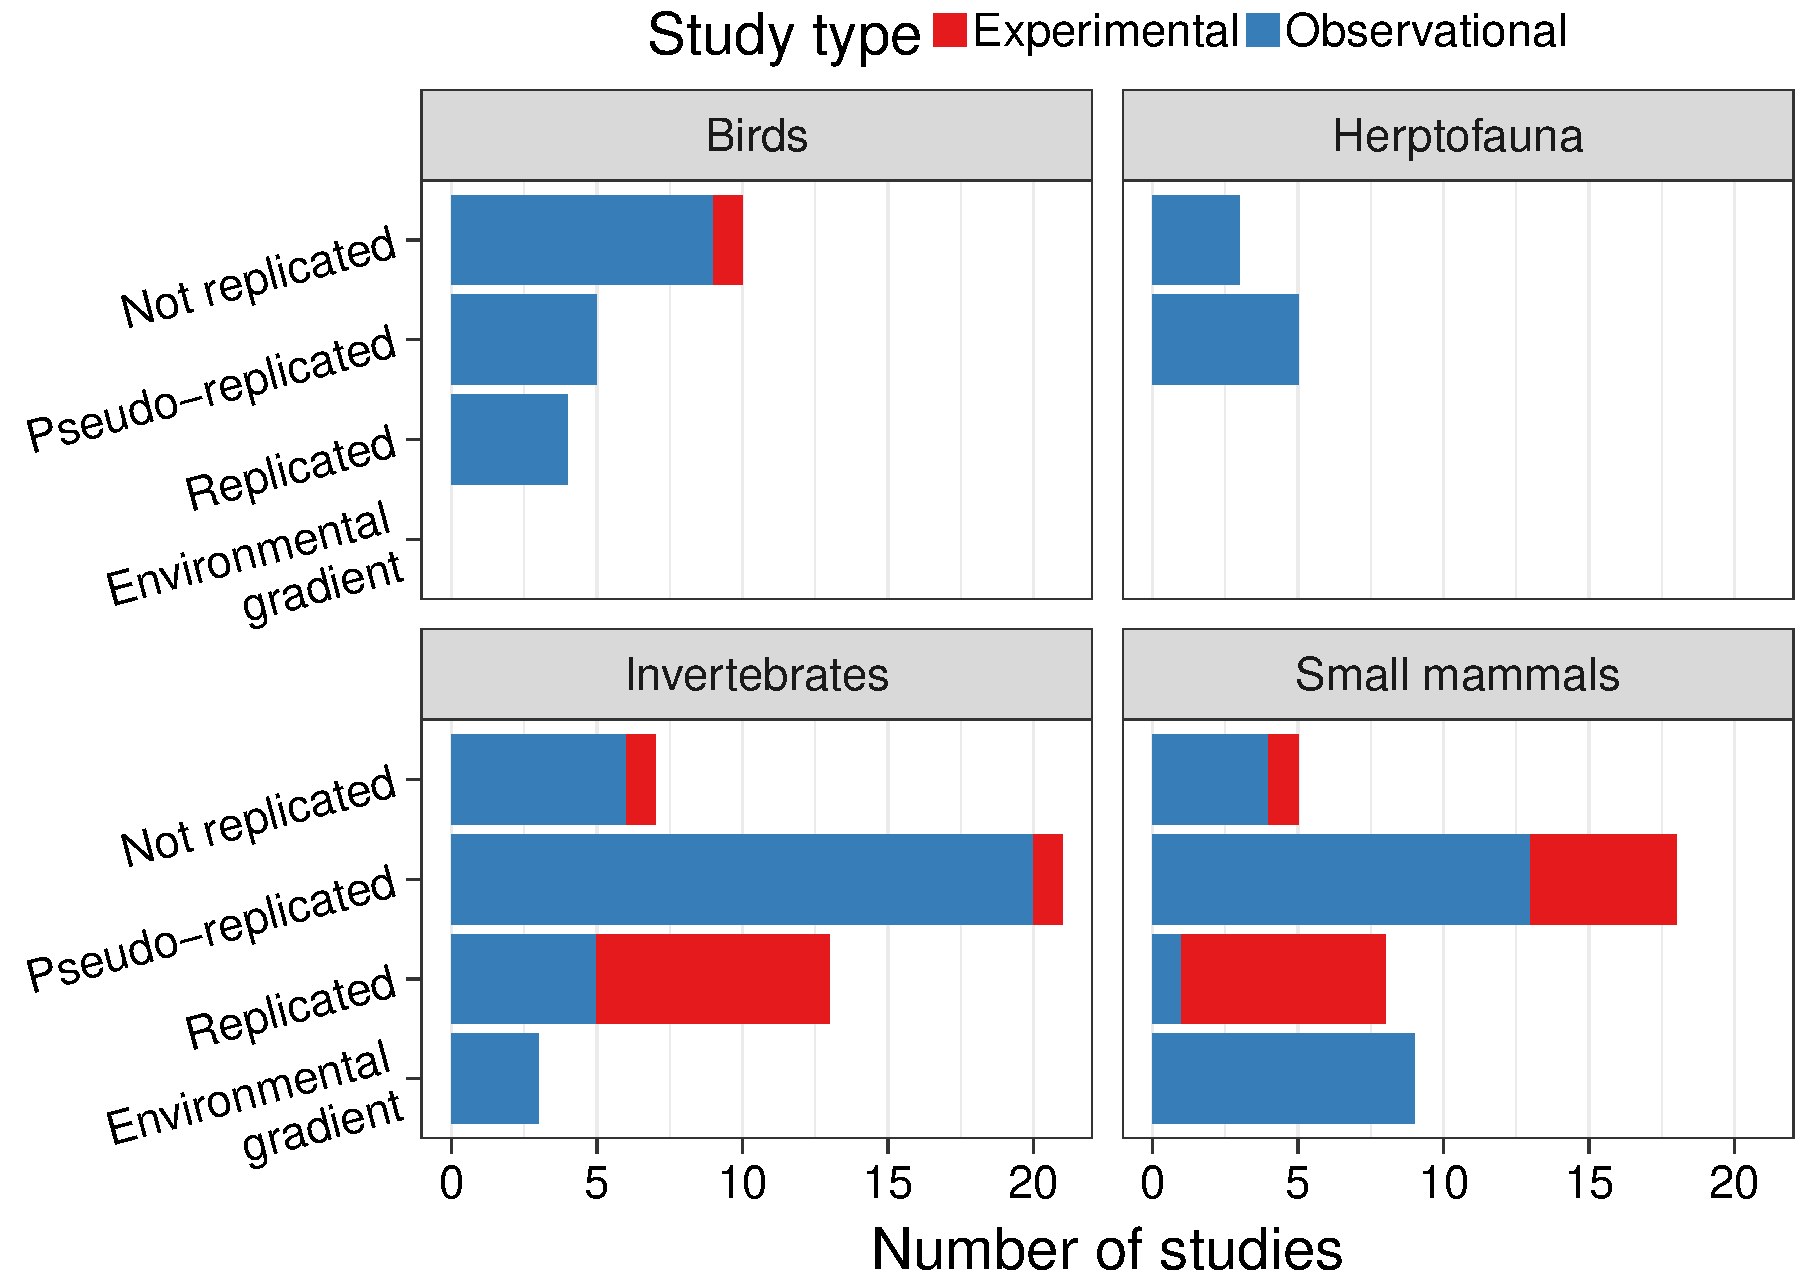
\includegraphics[width=\maxwidth]{figure/beamer-study_types-1} \hfill{}

\caption[ Number of studies per taxa, by study type]{ Number of studies per taxa, by study type}\label{fig:study_types}
\end{figure}


\end{knitrout}


\end{column}%
\end{columns}

%--------------------------
\begin{columns}[t,totalwidth=\twocolwid] % Split up the two columns wide column again




\begin{column}{0.6\textwidth} % The first column within column 2 (column 2.1
%\large\textbf{Most frequent response variables:}
%\color{blue}\rule{\linewidth}{1pt}
\begin{alertblock}{Response variables \& statistics}
 \normalsize
 \raggedright
\begin{itemize}
\item Most studies collected data on species abundance (Below)
\item Many also used these data for community analysis (Right)
\item Richness \& diversity indices are common, but they ignore species identity \& fail to detect different assemblages
\item Multivariate stats allow testing groups \& gradients, but most ordinations simply plotted groups differently.
\end{itemize}
 \end{alertblock} 
 \begin{figure}\caption{Relative frequency of response variables reported at least twice}
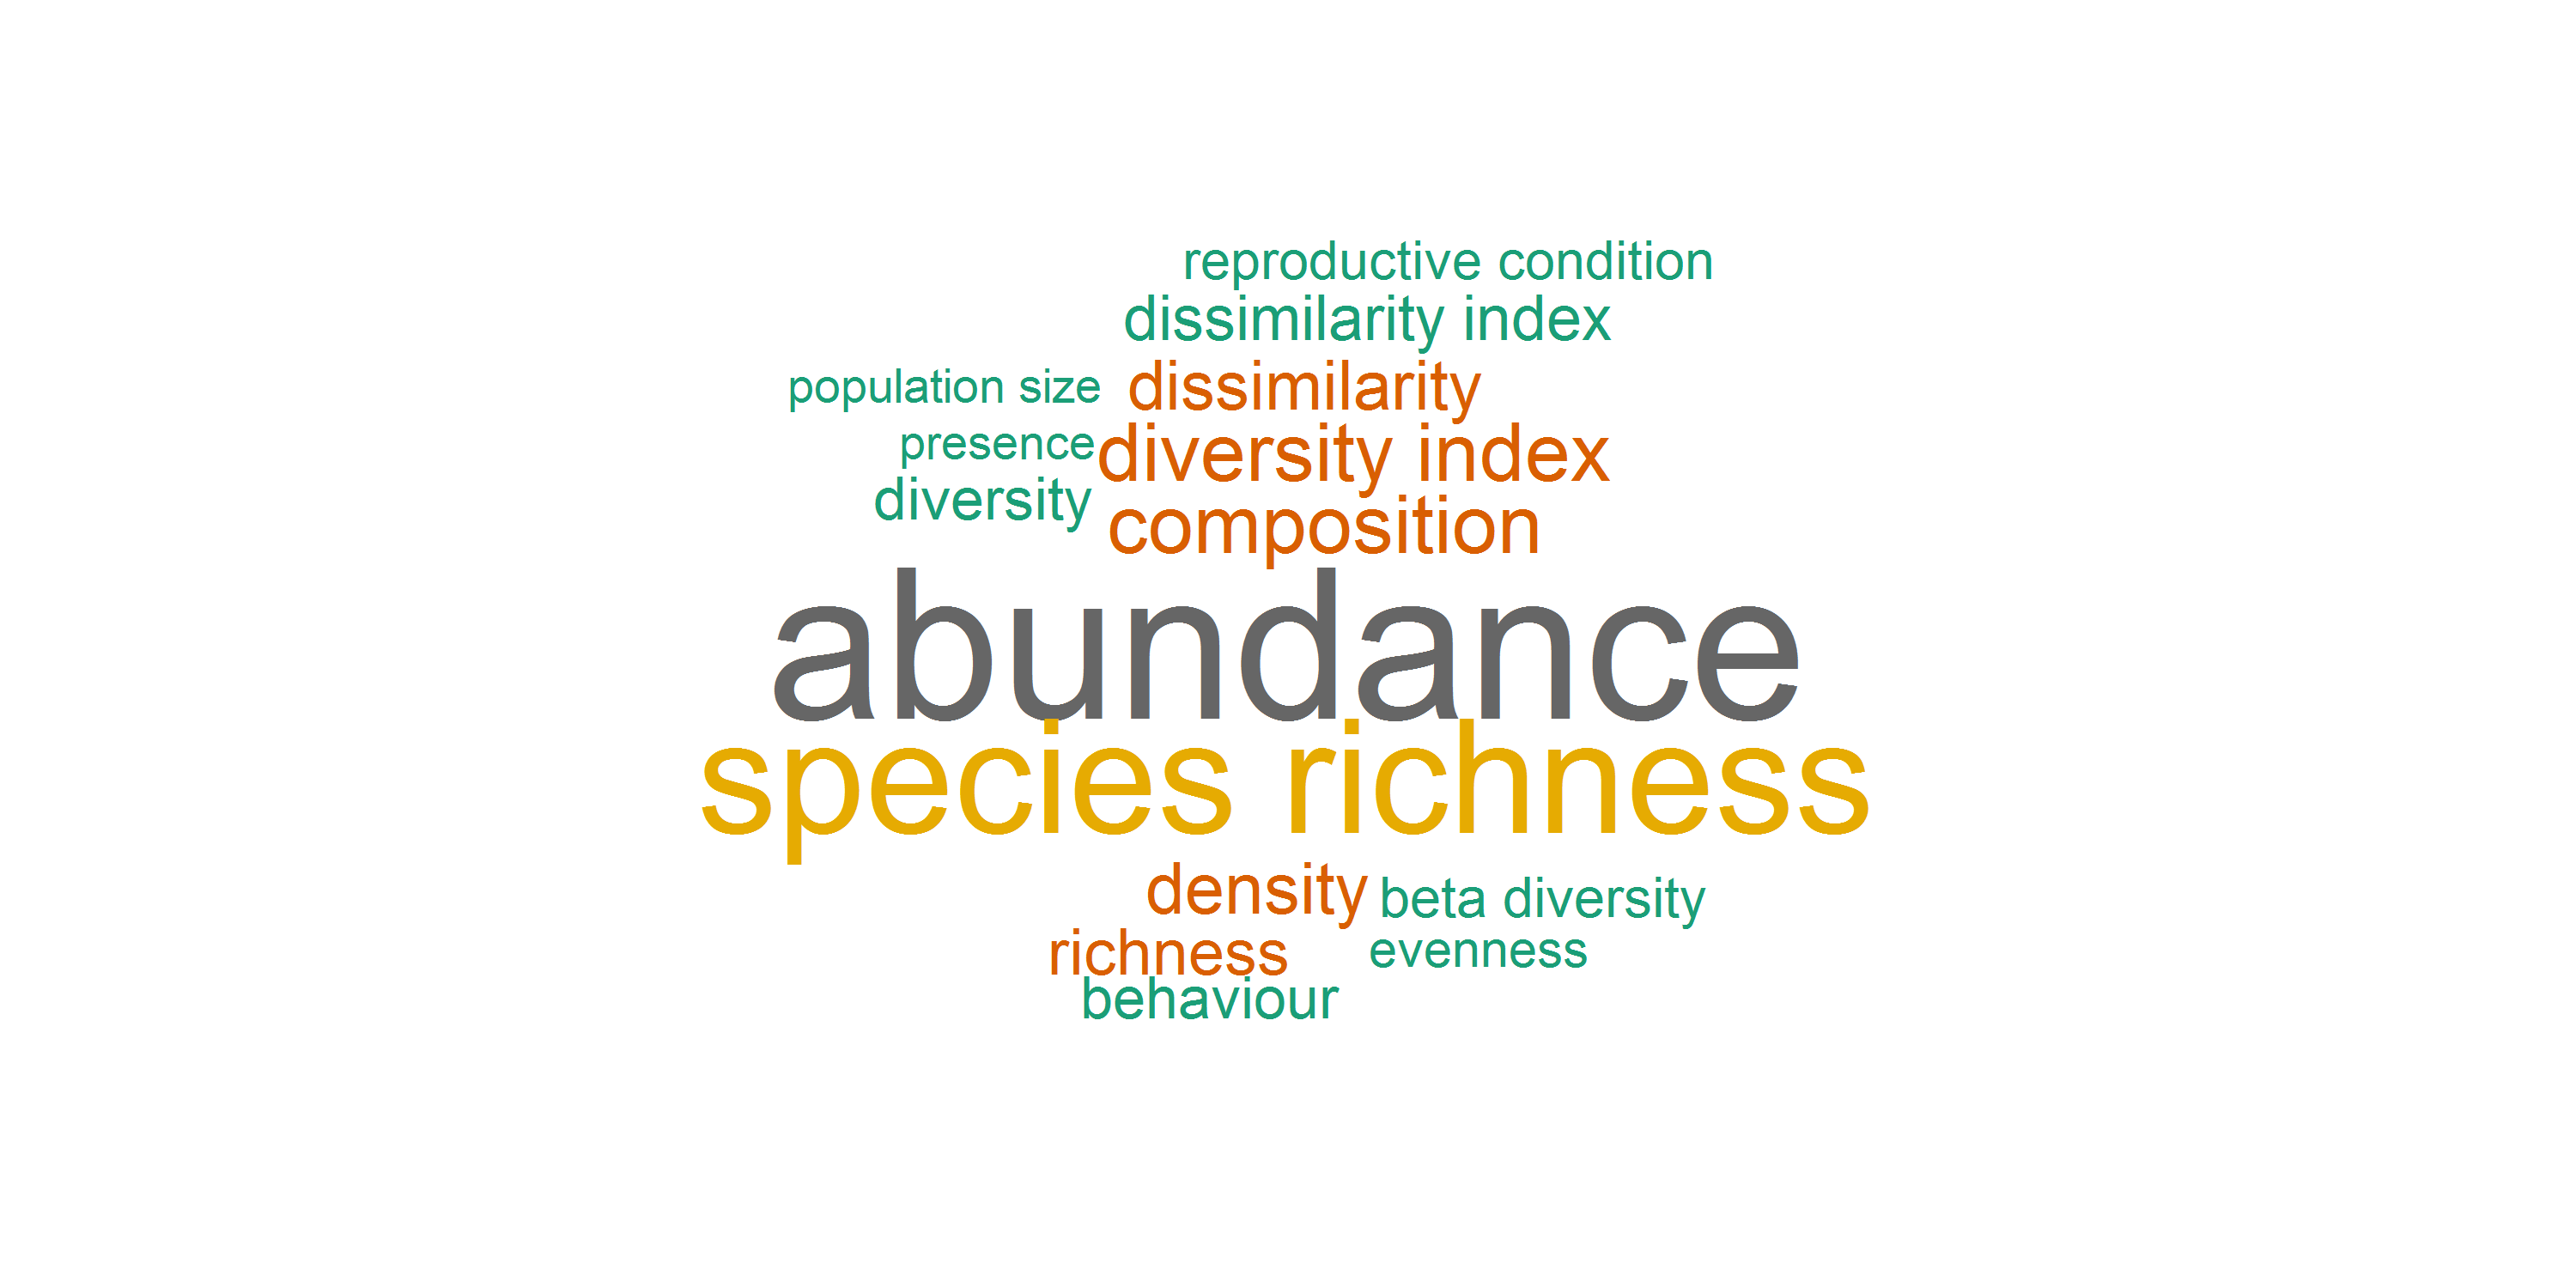
\includegraphics[trim=6.5cm 2cm 6.5cm 2cm, clip, width=0.98\linewidth]{figure/responses_wc}
\end{figure}

\end{column} % End of column 2.1

\begin{column}{0.38\textwidth} % 2.2
%\large\textbf{Most frequent response variables:}
\vspace{-1cm}
\begin{block}{Data analysis}
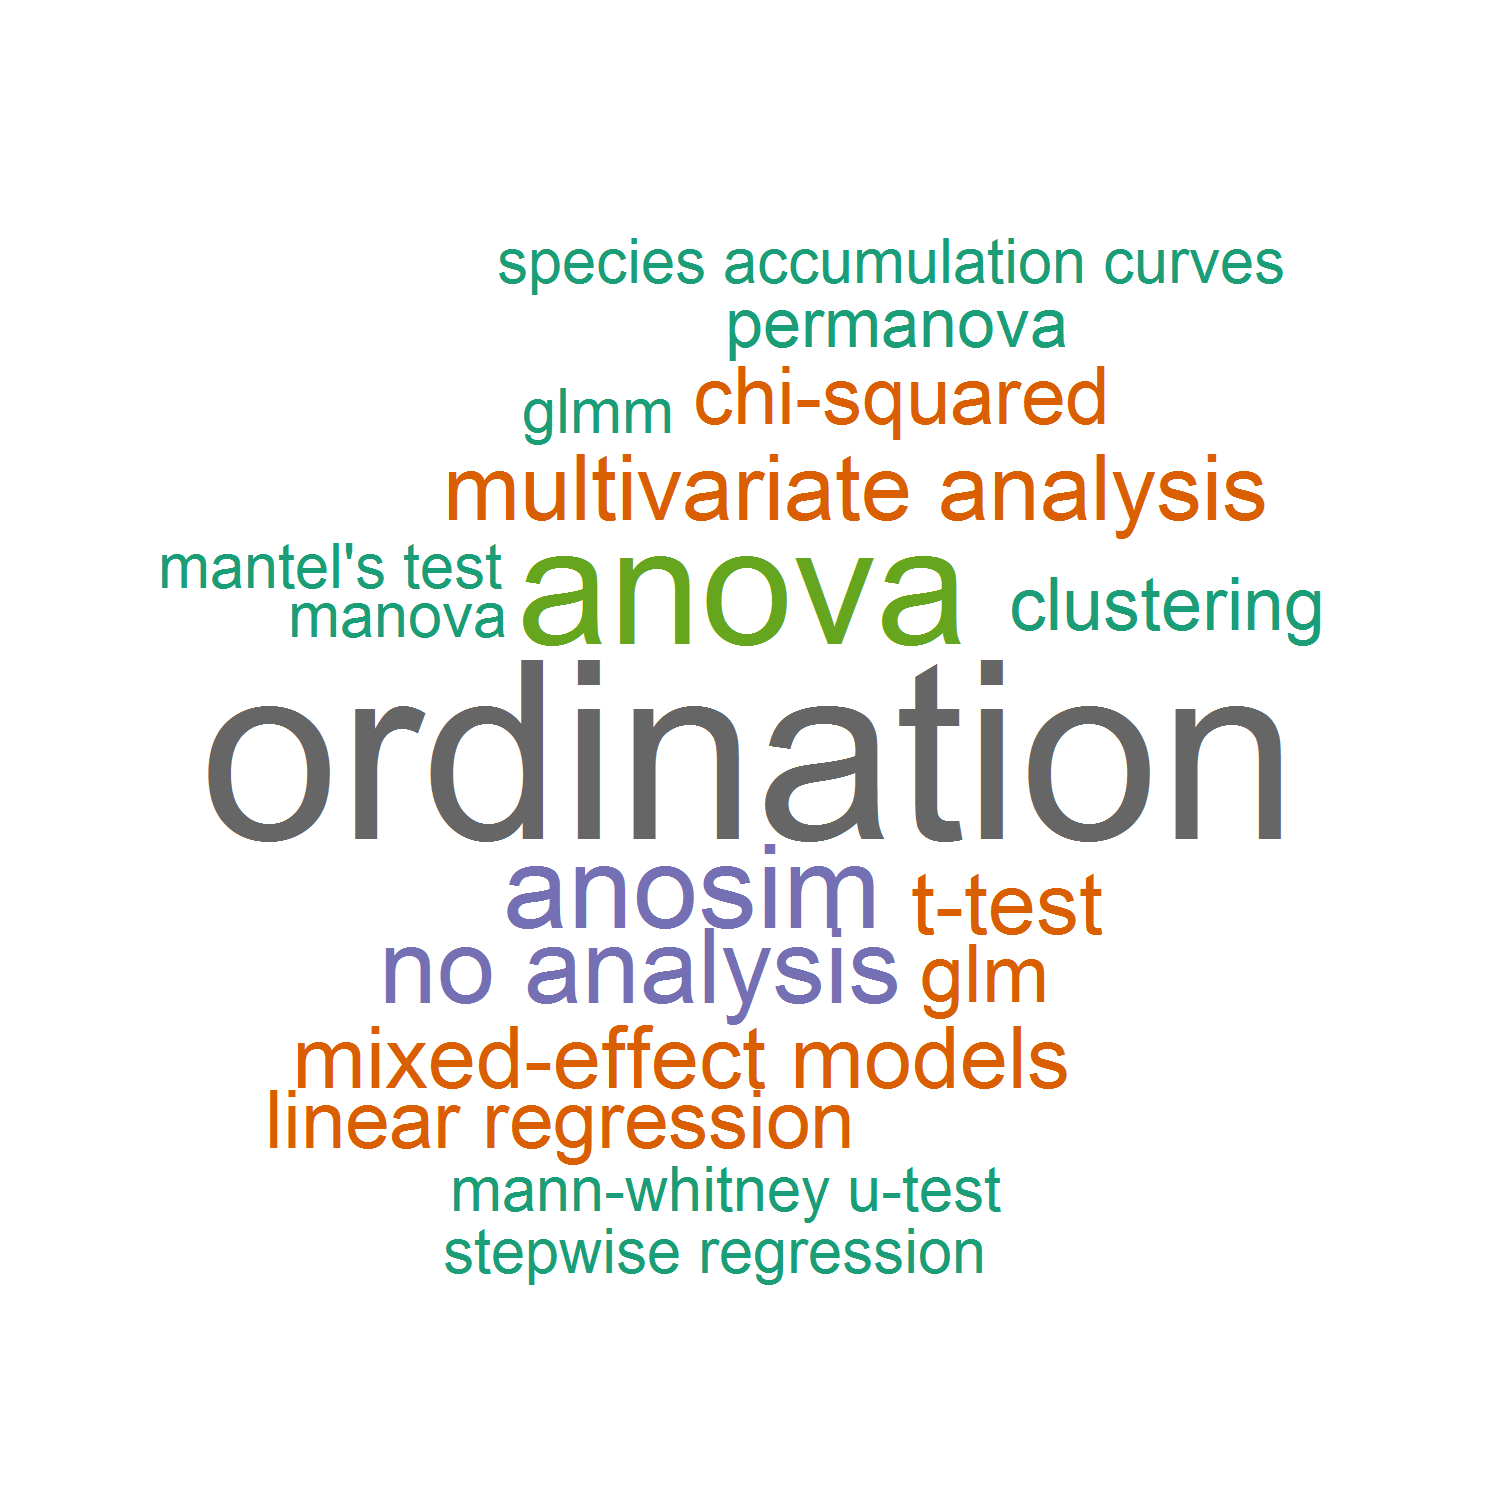
\includegraphics[trim=1.2cm 1cm 1.5cm 2cm, clip, width=1\linewidth]{figure/analyses_wc} 

\begin{knitrout}
\definecolor{shadecolor}{rgb}{0.969, 0.969, 0.969}\color{fgcolor}

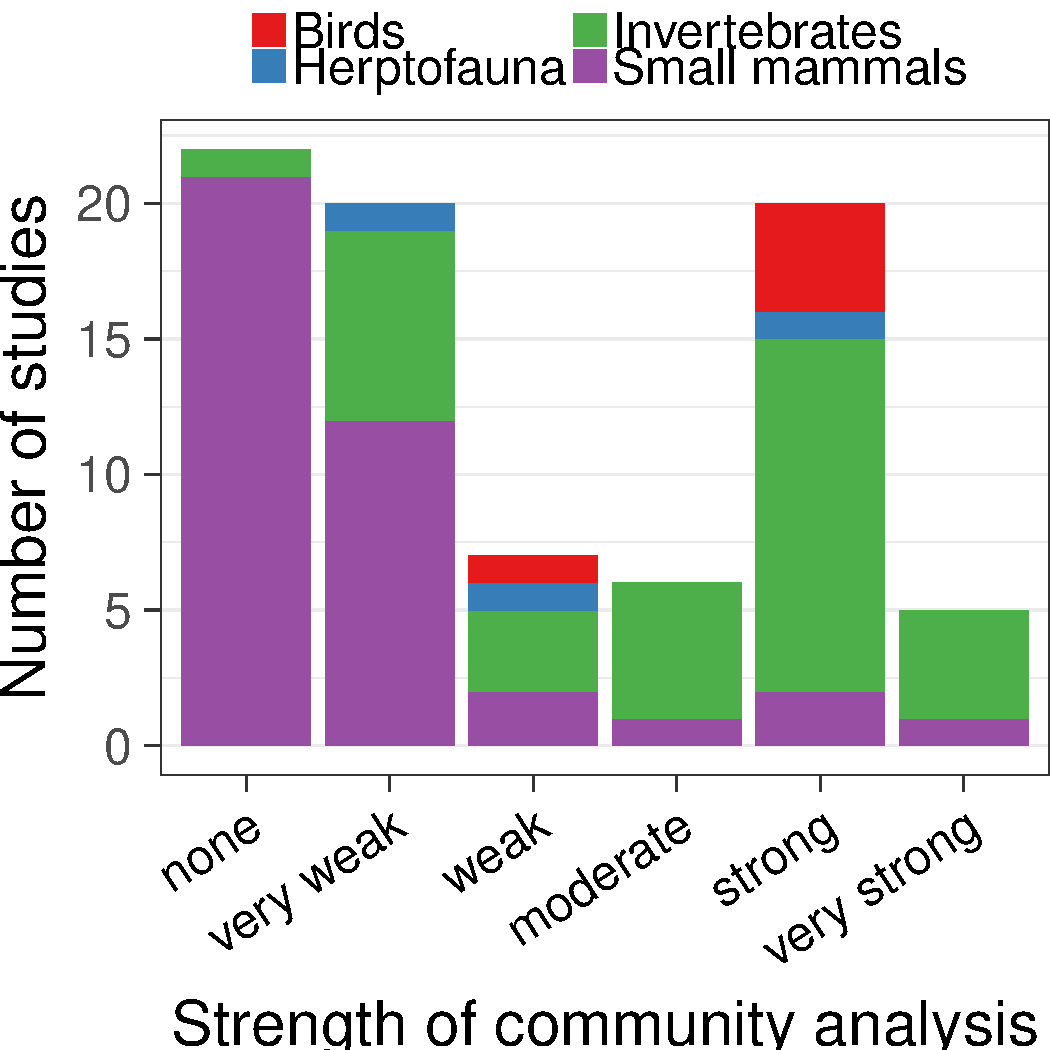
\includegraphics[width=\maxwidth]{figure/beamer-strength-1} \hfill{}



\end{knitrout}

\end{block}
\end{column} % End of column 2.2
\end{columns} % End of the split of column 2


\end{column} % End of the second column

\begin{column}{\sepwid}\end{column} % Empty spacer column

\begin{column}{\onecolwid} % The third column

\setbeamercolor{block alerted title}{fg=white,bg=BrewerRed1} % Change the alert block title colors
\setbeamercolor{block alerted body}{fg=black,bg=white} % Change the alert block body colors

\begin{alertblock}{\textbf{Biodiversity research lacks attention to heterogeneity \& variability}}

\begin{itemize}
\item Ecosystem theory and managment worldwide recognise role of spatial heterogeneity (\& variability in time) in enhancing biodiversity. 
\item Managers can create niche diversity and increase compositional diversity with spatially-patchy disturbance, \textbf{but the heterogeneity perspective in Africa is missing}.
\item Many data types familiar to researchers in Africa support heterogeneity-based analysis, but longer studies and multivariate analyses are required.
\end{itemize}

\end{alertblock}

Heterogeneity is rarely a research focus:

\begin{knitrout}
\definecolor{shadecolor}{rgb}{0.969, 0.969, 0.969}\color{fgcolor}

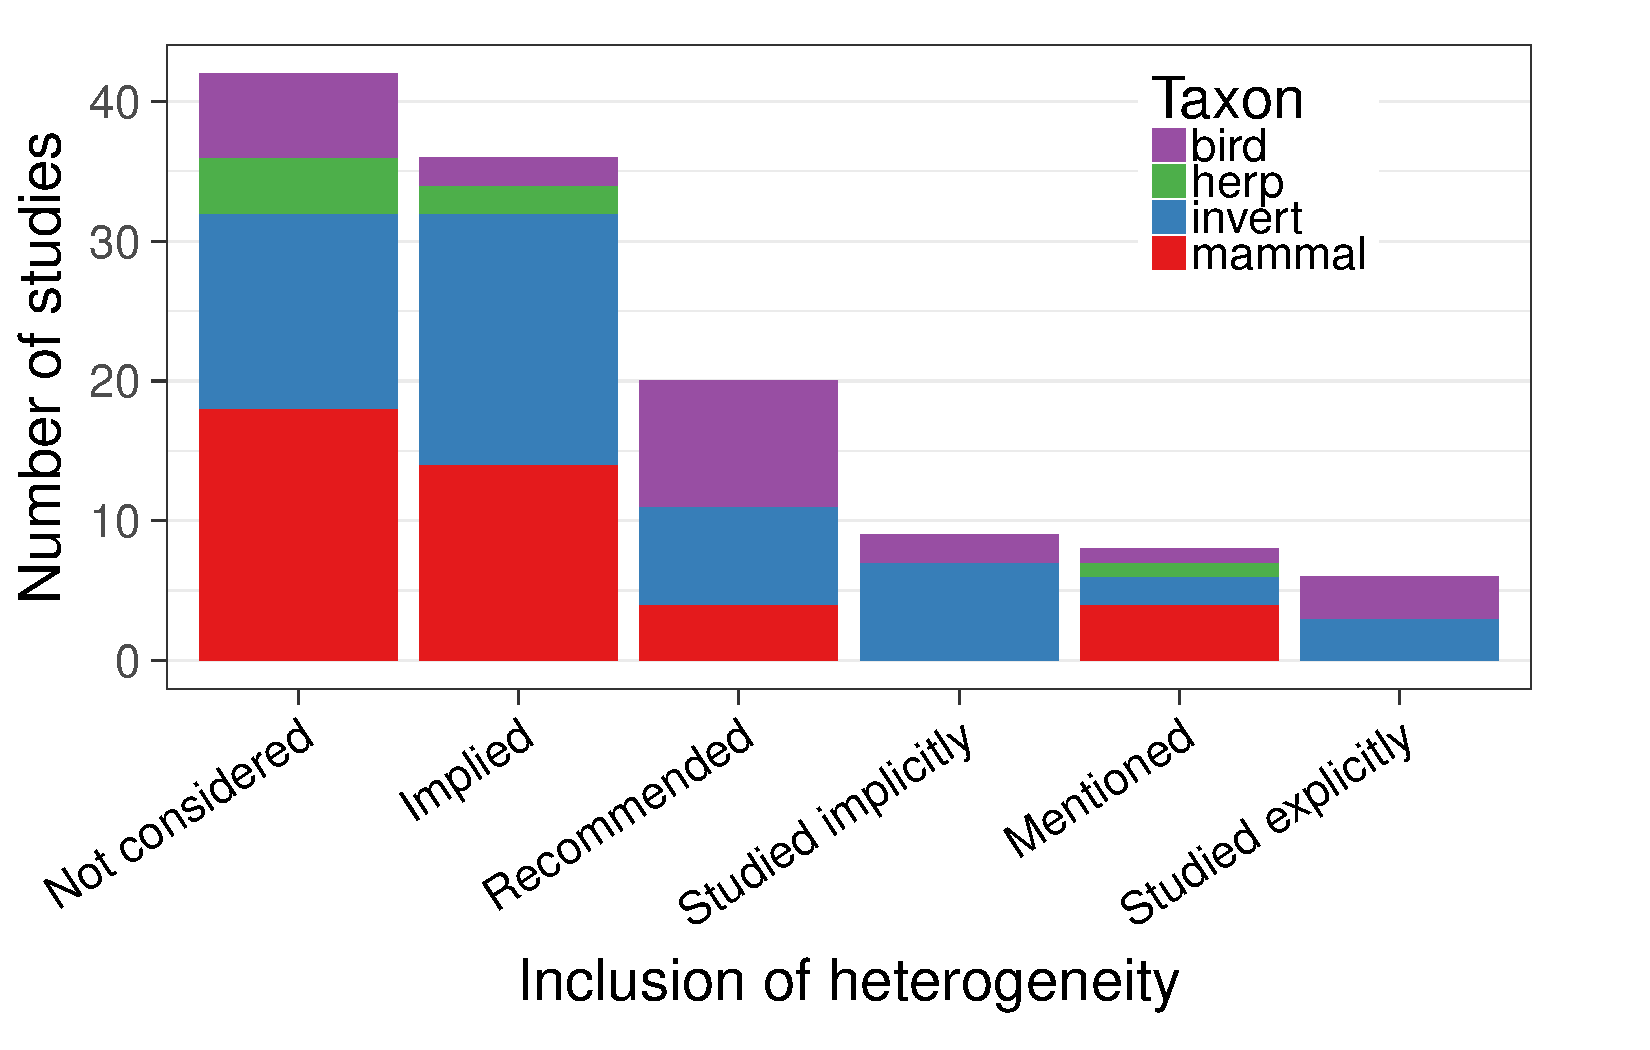
\includegraphics[width=\maxwidth]{figure/beamer-heterogeneity-1} \hfill{}



\end{knitrout}
\vspace{-1cm}
Above: We scored studies by whether they had a heterogeneity component, and if so, whether it was an explicit part of the study or could be inferred by a reader familiar with heterogeneity concepts.

\vskip 1cm

Most studies are too short to show temporal patterns:

\begin{knitrout}
\definecolor{shadecolor}{rgb}{0.969, 0.969, 0.969}\color{fgcolor}

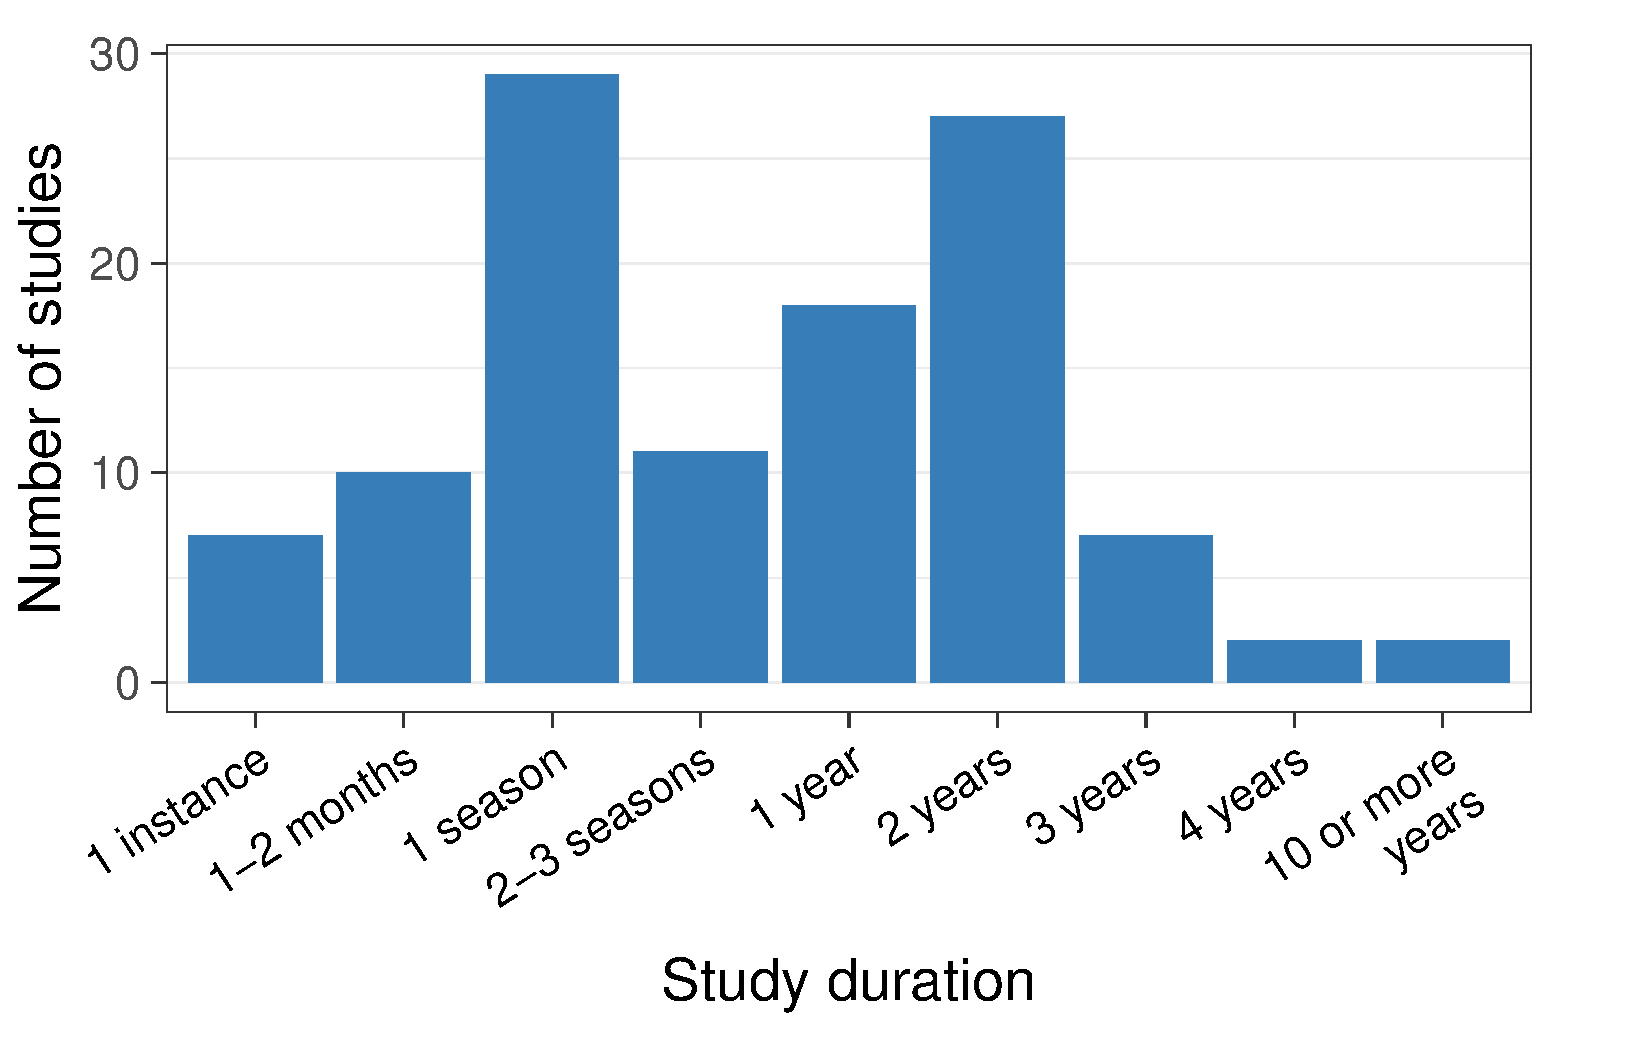
\includegraphics[width=\maxwidth]{figure/beamer-duration-1} \hfill{}



\end{knitrout}
\vskip 1cm 



\setbeamercolor{block alerted title}{fg=white,bg=BrewerBlue1} % Colors of the highlighted block titles
\setbeamercolor{block alerted body}{fg=black,bg=dblue!10}


\end{column} % End of the third column

\end{columns} % End of all the columns in the poster

\end{frame} % End of the enclosing frame

\end{document}
